\documentclass[11pt,a4paper]{article}
\usepackage[hyperref]{acl2017}
\usepackage{url}
\usepackage{times}
\usepackage{latexsym}
\usepackage{amsmath}
\usepackage{float}
\usepackage{svg}

% Please remember to install inkscape and include --shell-escape when
% using pdflatex:
% sudo apt-get install inkscape
% pdflatex --shell-escape sling

% Figures:
% https://docs.google.com/a/ringgaard.com/presentation/d/1QlQnyeG5UbUDEi2x9rxxjCXRQ1Qz9qjaTz__NWX-n8o/edit?usp=sharing

\floatstyle{boxed}
\restylefloat{figure}

%\aclfinalcopy
\def\confidential{DRAFT COPY.  DO NOT DISTRIBUTE.}

\title{SLING: A framework for frame semantic parsing}

\author{
Michael Ringgaard \\ Google Inc. \\ {\tt ringgaard@google.com} \\\And
Rahul Gupta \\ Google Inc. \\ {\tt grahul@google.com} \\\And
Fernando C. N. Pereira \\ Google Inc. \\ {\tt pereira@google.com} \\
}

\begin{document}
\maketitle

\begin{abstract}
We describe SLING, a framework for parsing natural language into
semantic frames. SLING supports general transition-based, neural-network parsing with
bi-directional LSTM input encoding and a Transition Based Recurrent
Unit (TBRU) for output decoding. The parsing model is
trained end-to-end using only the text tokens as input. The
transition system has been designed to output frame graphs directly without
any intervening symbolic representation.
The SLING framework includes an efficient and scalable frame store
implementation as well as a neural network JIT compiler for fast inference during parsing.
SLING is implemented in C++ and it is available for download on GitHub.
\end{abstract}

\section{Introduction}

Recent advances in machine learning make it practical to train
recurrent multi-level neural network classifiers, allowing us to rethink the
design and implementation of natural language
understanding (NLU) systems.

Earlier machine-learned NLU systems were commonly organized as pipelines of
separately trained stages for syntatic and semantic annotation of text.
A typical  pipeline would start with part-of-speech (POS) tagging, followed by
constituency or dependency parsing for syntactic analysis.
Using the POS tags and parse trees as feature inputs, later stages in the pipeline could then
derive semantically relevant annotations such as entity and concept mentions, entity types, coreference relationships,
and semantic roles (SRL).

For simplicity and efficiency, each stage in a practical NLU pipeline would just output its best hypothesis
and pass it on to the next stage~\cite{finkel2006}.
Obviously, errors could then accumulate
throughout the pipeline making it much harder for the system to perform
accurately. For instance, F1 on SRL drops by more than 10\% when going from gold to
system parse trees~\cite{toutanova2005}.

However, applications may not need the intermediate annotations produced
by the earlier stages of a NLU pipeline, so it would be preferable if all stages
could be trained together to optimize an objective based on the output
annotations needed for a particular application.

Earlier NLU pipelines often used linear classifiers for each stage.
Linear classifiers achieve simplicity and training efficiency at the expense of
feature complexity, requiring elaborate feature
extraction, many different feature types, and
feature combinations to achieve reasonable accuracy.
With deep learning, we can use embeddings, multiple layers, and recurrent
network connections to reduce the need for complex
feature design. The internal learned representations in model hidden layers
replace the hand-crafted feature combinations and intermediate representations
in pipelined systems.


The SLING parser exploits deep learning to bypass those limitations of classic pipelined systems.
It is a transition-based parser that outputs frame graphs directly without any
intervening symbolic representation (see Section~\ref{sec:ts}). Transition-based
parsing is often associated with dependency parsing, but we have designed a
specialized transition system that outputs frame graphs instead of dependency
trees.

We use a recurrent feed-forward unit for predicting the actions in the
transition sequence, where the hidden activations from predicting each
transition step are fed back into subsequent steps.
A bidirectional LSTM is used for encoding the input (Figure~\ref{fig:network}).
This neural network architecture has been implemented using DRAGNN~\cite{dragnn}
and TensorFlow~\cite{tensorflow}.

The SLING framework and a semantic parser built in it are now available as open-source code in GitHub.\footnote{\url{https://github.com/google/sling}}

In Section~\ref{sec:framesem} we introduce \emph{frame semantics}, the linguistic theory that
inspired SLING, as well as the SLING frame store, a
C++ framework for representing and storing semantic frames compactly and
efficiently.
Section~\ref{sec:att} introduces the parser's frame-semantics-oriented attention mechanism, and
Section~\ref{sec:ts} describes the transition system used for producing
frame graphs. Section~\ref{sec:features} describes the features used by the
parser.

\begin{figure*}[t]
  \centering
  \includesvg{network}
  \caption{Neural network architecture of the SLING parser. The input is encoded by
  a bi-directional LSTM and fed into a recurrent
  feed-forward (FF) unit that proposes transition system actions.
  The hidden layer activations and the transition system state are combined to create
  the input feature vector for the next step. The FF unit is
  run repeatedly until the transition system has reached a final state.}
  \label{fig:network}
\end{figure*}

\section{Frame semantics}
\label{sec:framesem}

While frames in SLING are not tied to any particular linguistic theory or
knowledge ontology, they are inspired by \emph{frame semantics}, the
theory of linguistic meaning originally developed by Charles Fillmore~\cite{fillmore1982}.
Frame semantics connects linguistic semantics to encyclopedic knowledge, with the
central idea that understanding the meaning of a word requires access to all
the essential knowledge that relates to that word. A word \emph{evokes} a frame
representing the specific concept it refers to.

A semantic frame is a set of statements that give "characteristic
features, attributes, and functions of a denotatum, and its characteristic
interactions with things necessarily or typically associated with it."~\cite{alan2001}.
A semantic frame can also be viewed as a coherent group of concepts
such that complete knowledge of one of them requires knowledge of all of them.

Frame semantics is not just for individual concepts, but can be generalized
to phrases, entities, constructions, and other larger and more complex linguistic
and ontological units. Semantic frames can be also used in information modeling
for constructing knowledge bases of world knowledge and common sense, and frame
semantics can also form the basis for reasoning about
metaphors~\cite{narayanan1999},
metonymy,
actions~\cite{narayanan1999reasoning},
or perspective~\cite{chang2002}.

\section{Frames in SLING}
\label{sec:slingframes}

At a more technical level, a SLING frame consists of a list of slots, where each
slot has a name (role) and a value. The slot values can be literals like numbers
and strings, or links to other frames. The frames essentially form a directed graph where
the frames are the (typed) nodes and the slots are the labeled edges. A frame
graph can also be viewed as a feature structure~\cite{carpenter2005} and
unification can be used for induction of new frames from existing frames.
Sometimes it is also useful to use frames for representing more basic data
structures like a C struct with fields, a JSON object, or a record in a
database.

SLING frames live inside a \emph{frame store}. A store is a container that
tracks all the frames that have been allocated in the store, and serves as a
memory allocation arena for them. When making a new frame, one
specifies the store where the frame should be allocated. The frame will live in
this store until the store is deleted or the frame is garbage collected because
there no remaining live references to it.\footnote{See the \href{https://github.com/google/sling/blob/master/frame/README.md}{SLING Guide}
for a detailed description of the SLING frame store implementation.}

SLING frames are externally represented in a superset of JSON that allows references
between frames (JSON objects) with the {\tt \#n} syntax. Frames can be
assigned identifiers (\emph{ids}) using the {\tt=\#n} syntax. SLING frames can have both numeric and
named ids and both slot names and values can be frame references. Where JSON
objects can only represent trees, SLING frames can be used for representing
arbitrary graphs. SLING has special syntax for built-in slot names:

\begin{table}[h!]
\begin{tabular}{|l|l|l|}
\hline
Syntax & Symbol & RDF \\
\hline
=name & id:name & rdf:ID \\
:name & isa:name & rdf:InstanceOf \\
+name & is:name & rdfs:subClassOf \\
\hline
\end{tabular}
\end{table}

Documents are also represented using frames, where the document frame has slots
for the document text, the tokens, and the mention phrases and the frames they
evoke. See Figure~\ref{fig:slingdoc} for an example.

\begin{figure*}[t]
  \begin{verbatim}
{
  :/s/document
  /s/document/text: "John hit the ball"
  /s/document/tokens: [
    {/s/token/text: "John" /s/token/start: 0  /s/token/length: 4},
    {/s/token/text: "hit"  /s/token/start: 5  /s/token/length: 3},
    {/s/token/text: "the"  /s/token/start: 9  /s/token/length: 3},
    {/s/token/text: "ball" /s/token/start: 13 /s/token/length: 4}
  ]
  /s/document/mention: {
    :/s/phrase /s/phrase/begin: 0
    /s/phrase/evokes: {=#1 :/saft/person }
  }
  /s/document/mention: {
    :/s/phrase /s/phrase/begin: 1
    /s/phrase/evokes: {
      :/pb/hit-01
      /pb/arg0: #1
      /pb/arg1: #2
    }
  }
  /s/document/mention: {
    :/s/phrase /s/phrase/begin: 3
    /s/phrase/evokes: {=#2 :/saft/consumer_good }
  }
}
\end{verbatim}
  \caption{The text ``John hit the ball" in SLING frame notation. The document
  itself is represented by a frame that has the text, an array of tokens and
  the mentions that evoke frames. There are three frames: a person frame (John),
  a consumer good frame (bat) and a hit-01 frame. The hit frame has the person
  frame as the agent (arg0) and the ball frame as the object (arg1).}
  \label{fig:slingdoc}
\end{figure*}

\section{Attention}
\label{sec:att}

The SLING parser is a kind of sequence-to-sequence model that first encodes the
input text token sequence with a biLSTM encoder and then runs the transition
system on that encoding to produce a sequence of transitions, where each transition
updates the system state that combined with the input encoding form the input for
the transition feed-forward cell that predicts the next transition (Figure~\ref{fig:network}).

Sequence-to-sequence models often rely on an ``attention" mechanism to focus
the decoder on the parts of the input most relevant for producing the next output
symbol. In this work, however, we use a somewhat difference attention mechanism,
loosely inspired on neuroscience models of attention and awareness
~\cite{nelson2017,graziano2013}. In our model, attention focuses on parts of the frame
representation that the parser has created so far, rather than focusing on (encodings of)
input tokens as is common for other sequence-to-sequence attention mechanisms.

We maintain an \emph{attention buffer} as part of the transition system state.
This an ordered list of frames, where the order represents closeness to the center
of attention. Transition actions maintain the attention buffer, bringing a frame
to the front when the frame
is evoked or re-evoked by the input text. When a new frame is evoked, it will
merge the concept and its roles into a new coherent chunk of meaning, which is
represented by the new frame and its relations to other frames, and this will
become the new center of attention. Our hypothesis is that by maintaining this
attention mechanism, we only need to look at a few recent frames brought into
attention to build up the desired frame graph.

\section{Transition system}
\label{sec:ts}

In the parsing literature, \emph{transition systems} have been
used to construct dependency parse trees from a sequence of state-action pairs
$(s_i,a_i)$. The transition system takes a state $s_i$ and an action $a_i$ and
constructs a new state $s_{i+1}$. This allows you to build a tree structure by
predicting a sequence of actions. For example, the \emph{arc-standard}
transition system \cite{nivre2006} uses {\bf SHIFT}, {\bf LEFT-ARC(label)}, and
{\bf RIGHT-ARC(label)} actions to construct a dependency parse tree from a
sequence of those actions.

We use the same idea to construct a frame graph where frames can be
evoked by phrases in the input. Instead of using a stack, we have the attention buffer introducted
in the previous section, which keeps track of the most salient frames in the
discourse. The front of the attention buffer serves as the working memory for
the parser, which operates on those frames. The transition system simultaneously
build the frame graph and maintain the attention buffer.
The current transition system consists of the following actions:

\begin{itemize}
  \item {\bf SHIFT} -- Moves to next input token. Only valid when not at the
        end of the input buffer.
  \item {\bf STOP} -- Signals that we have reach the end of the parse. This is
        only valid when at the end of the input buffer. Multiple STOP actions
        can be added to the transition sequence, e.g. to make all sequences in a
        beam have the same length. After a STOP is issued, no other actions are
        permitted except more STOP actions.
  \item {\bf EVOKE(type, n)} -- Evokes frame of with type {\bf type} from
        the next {\bf n} tokens in the input. The evoked frame becomes the new
        center of attention.
  \item {\bf REFER(frame, n)} -- Makes a new mention of the next {\bf n} tokens
        in the input evoking an existing frame in the attention buffer. This
        frame will become the new center of attention.
  \item {\bf CONNECT(source, role, target)} -- Adds slot to {\bf source} frame
        in the attention buffer with name {\bf role} and value {\bf target}
        where {\bf target} is an existing frame in the attention buffer. The
        {\bf source} frame become the new center of attention.
  \item {\bf ASSIGN(source, role, value)} -- Adds slot to {\bf source} frame in
        the attention buffer with name {\bf role} and constant value {\bf value}
        and moves the frame to the center of attention. The {\bf ASSIGN} action
        is used for assigning a constant value to a slot in contrast to
        {\bf CONNECT} where the value is another frame in the attention buffer.
  \item {\bf EMBED(target, role, type)} -- Creates a new frame with
        type {\bf type} and add a slot to it with name {\bf role} and value
        {\bf target} where {\bf target} is an existing frame in the attention
        buffer. The new frame becomes the new center of attention.
  \item {\bf ELABORATE(source, role, type)} -- Creates a new frame with type
        {\bf type} and adds a slot to an existing frame {\bf source} in the
        attention buffer with {\bf role} set to the new frame. The new frame
        becomes the new center of attention.
\end{itemize}

In summary, {\bf EVOKE} and {\bf REFER} are used to evoke frames from text
mentions, while {\bf ELABORATE} and {\bf EMBED} are used to create frames not
directly evoked by text.

This transition system can generate any connected frame graph where the frames
are either directly on indirectly evoked by mention phrases in the text. A frame
can be evoked by multiple mentions and the graph can have cycles.

The transition system can potentially have an unbounded number of actions since
it is parameterized by phrase length and attention buffer indices with can be
arbitrarily large, so in the current implementation, we only consider the
top $k$ frames in the attention buffer $(k=5)$ and do not consider phrases
longer than those in the training copus.

Multiple transition sequences can generate the same frame annotations, but we
have implemented an oracle sequence generator that takes a document and converts
it to a canonical transition sequence in a way similar to how this is done
for transition-based dependency parsing \cite{nivre2006}, e.g. the sentence
``John hit the ball" will generate the following transition sequence:
\begin{verbatim}
  EVOKE(/saft/person, 1)
  SHIFT
  EVOKE(/pb/hit-01, 1)
  CONNECT(0, /pb/arg0, 1)
  SHIFT
  SHIFT
  EVOKE(/saft/consumer_good, 1)
  CONNECT(1, /pb/arg1, 0)
  SHIFT
  STOP
\end{verbatim}

\section{Features}
\label{sec:features}

The LSTMs only uses lexical features based on the current input word:

\begin{itemize}
  \item The current word itself. During training we initialize the embeddings
  for this feature with pre-trained word embeddings \cite{mikolov2013} for all
  the words in the vocabulary collected from the training data.
  \item The prefixes and suffixes of the current input word. We only use
  prefixes up to three characters in our experiments.
  \item Word shape features based on the characters in the current input word:
  hyphenation, capitalization, punctuation, quotes, and digits. Each of these
  features has its own embedding matrix.
\end{itemize}

The TBRU is a simple feed-forward unit with a single hidden layer.
It takes the hidden activations from the LSTMs as well as the activations from
the hidden layer from the previous steps as raw input features, and maps them
through embedding matrices to get the input vector for the  hidden layer. The
raw input features used are:

\begin{itemize}
  \item The hidden activations from the left-to-right and right-to-left LSTMs
  for the current token in the parser state.
  \item The attention feature looks at the top-5 frames in the attention buffer
  and finds the phrases in the text (if any) that evoked them. The activations
  from the left-to-right and right-to-left LSTMs for the last token in these
  phrases are used as input features. These serve as the continuous lexical
  representations of the top frames in the attention buffer.
  \item The hidden layer activations of the transition steps which evoked or
  brought into focus the top-5 frames in the attention buffer. These serves as a
  continuous representation of the semantic context for these frames, i.e. a
  representation of the state when these frames were evoked most recently.
  \item The history feature uses the hidden activations in the feed-forward
  unit from the previous five steps as feature inputs to the current step.
  \item The roles features extract the role edges between the top-5 frames in
  the attention buffer. These are triples of the form $(s_i, r_i, t_i)$ meaning
  that the frame at position $s_i$ in the attention buffer has a role $r_i$ with
  the frame at position $t_i$ in the attention buffer as its value. Back-off
  features are added for the source roles $(s_i,r_i)$, target role $(r_i, t_i)$,
  and unlabeled roles $(s_i,t_i)$.
\end{itemize}

\section{Experiments}

We used the OntoNotes corpus \cite{ontonotes2006} to construct a corpus
with frame semantic annotations for evaluating the parser. We took the
PropBank SRL layer \cite{palmer2005} and converted the predicate-argument
structures into frame annotations. We also annotated the corpus with
entity frames with entity types using a state-of-the-art entity tagger.
We determined the head token of each argument span and if this coincided
with the span of an existing frame, then we used it as the evoking span for the argument
frame, otherwise we just used the head token as the evoking span of the argument frame.

The various frame types mentioned above are listed in
Table~\ref{tab:types}. They include 7 conventional entity types,
6 top-level non-entity types (e.g. date), 13 measurement types, and
more than 5400 PropBank frame types. All the frame roles are collapsed onto
/pb/arg0, /pb/arg1, and so on. Our training corpus size was $111,006$ sentences = $2,206,274$ tokens.

\begin{table*}[t]
\begin{tabular}{|l|p{11cm}|}
\hline
{\bf Type set} & {\bf Details} \\
\hline
Entity types & /saft/\{person, location, organization, art, consumer\_good, event, other\} \\
\hline
Top-level non-entity types & /s/\{thing, date, price, measure, time, number\} \\
\hline
Fine-grained measure types & /s/measure/\{area, data, duration, energy, frequency, fuel, length, mass, power, speed, temperate, voltage, volume\} \\
\hline
PropBank SRL types & 5426 types, e.g. /pb/write-01, /pb/tune-02 etc.  \\
\hline
\end{tabular}
\caption{Details of the type-sets used in our experiments.}
\label{tab:types}
\end{table*}

\begin{table}[ht]
\begin{tabular}{|l|r|r|}
\hline
{\bf Action Type} & {\bf \# Unique Args} & {\bf Raw Count} \\
\hline
SHIFT & 1 & 2,206,274 \\
\hline
STOP & 1 & 111,006 \\
\hline
EVOKE & 5,532 & 1,080,365 \\
\hline
CONNECT & 1,421 & 635,734 \\
\hline
ASSIGN & 13 & 5,430 \\
\hline
{\bf Total} & 6,968 & 4,038,809 \\
\hline
\end{tabular}
\caption{Per transition-type statistics of the transitions used to generate the gold
frames in the OntoNotes training corpus.}
\label{tab:action-table}
\end{table}

Table~\ref{tab:action-table} presents the statistics of the transitions required
to generate the gold frames in the training corpus. As expected, we saw one SHIFT action
per training token, and one STOP action per training sentence.
We saw the EVOKE action take $5532$ unique (length, type) arguments in the corpus, for a
raw count of roughly $1.08$ million. Overall our action space had $6968$ actions, which is also
the size of the softmax layer of our TBRU decoder.


\noindent{{\bf Hyperparameters:}} Our final set of hyperparameters after performing a grid search
was: learning\_rate = $0.0005$, optimizer = Adam~\cite{kingma2014} with
$\beta_1 = 0.01, \beta_2 = 0.999, \epsilon = 1e-5$, no dropout, gradient clipping at $1.0$,
exponential moving average, no layer normalization, and a training batch size of $8$.

We stopped training after $120,000$ steps, where each step corresponds to processing one training batch,
and evaluated on the dev corpus ($15,084$ sentences) after every checkpoint (= $2,000$ steps). Figure~\ref{fig:dev-eval} shows the
how the various evaluation metrics evolve as training progresses. Section~\ref{sec:eval} contains
the details of these metrics are evaluated. We picked the checkpoint with the best `Slot F1`
score.

\begin{figure}
\centering
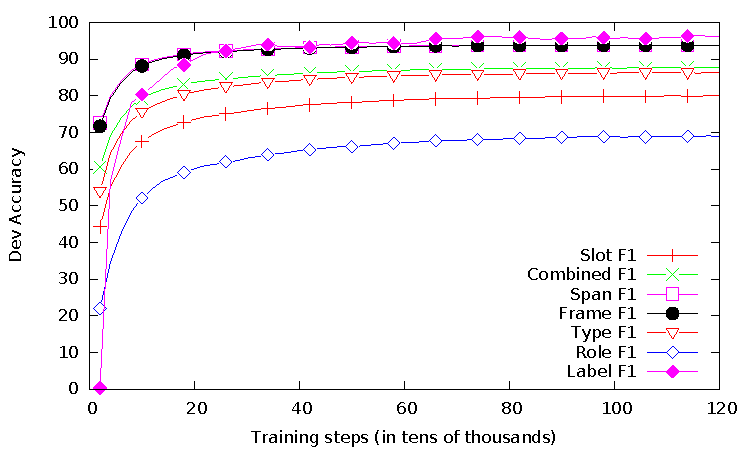
\includegraphics[width=\columnwidth]{dev-eval.pdf}
  \caption{Various frame graph accuracies over the dev set as training progresses.
	Training was stopped at $120,000$ iterations since we saw very little improvement after that.}
  \label{fig:dev-eval}
\end{figure}

\section{Evaluation}
\label{sec:eval}

An annotated document consists of a number of connected frames and as well as
phrases, i.e. token spans, evoking these frames. We evaluate the accuracy of the
annotations by comparing the generated frames with the gold standard frame
annotations from the evaluation corpus.

The documents are matched by constructing a virtual graph where the document
is the start node. The document node is then connected to the spans and the
spans are connected to the frames that the spans evoke. This graph is then
extended by following the frame-to-frame links via the roles. Accuracy is
computed by aligning the golden and predicted graphs and computing precision,
recall, and F1. These accuracies are separately computed for the spans, frames,
types of those frame, roles that link to other frames (referred to as 'roles'),
and roles that link to global constants (referred to as 'labels').

We also report two aggregates of the accuracies above: (a) {\em Slot}, which is
an aggregate of {\em Type}, {\em Role}, and {\em Label}, and (b) {\em Combined},
which is an aggregate of {\em Span}, {\em Frame}, {\em Type}, {\em Role}, and
{\em Label}.

We rate the checkpoints using the Slot-F1 metric and select the checkpoint that
has the best Slot-F1. Intuitively, a high {\em Slot} score reflects that the
right type of frames are being evoked, along with the right set of slots and links
to other frames.

In Figure~\ref{fig:dev-eval}, we can see that as training progresses,
the model learns to output the spans and frames evoked from those spans with a fairly
high accuracy (SPAN F1 $\approx$ FRAME F1 $\approx$ $94\%$). It also gets the
type of those frames right with a TYPE F1 of $= 86.26\%$. Our ROLE F1 though
is lower at just $68.98\%$. ROLE F1 measures the accuracy of correctly getting
the frame-frame link, including the label of the link. Some error analysis is required
to ascertain the aspect(s) of frame-frame links missed by the model. Also note that
currently the {\em roles} feature is the only one that captures inter-frame link information.
Augmenting this with more features should help improve ROLE accuracy, and we shall
consider investigating this in our future work. 

Finally, we take the best checkpoint (with SLOT F1 $= 79.95\%$ at $110,000$ steps),
and evaluate it over the test corpus. 
Table~\ref{tab:eval} lists the accuracy of this model on the test and dev corpora.
With the except of LABEL accuracies, all the other metrics exhibit less than half a percent
difference between the test and dev corpora. This illustrates that despite the lack of
dropout, the model hasn't overfit and generalizes well to unseen text. As far the disparity
on LABEL is concerned (LABEL F1 of $95.91$ on dev vs $93.82$ on test), we note that the LABEL
accuracies are the slowest to improve while training.
In Figure~\ref{fig:dev-eval}, we can see that LABEL F1 starts close to zero, and although it
improves to $95.91$, it still shows signs of further improvement when training was stopped,
in contrast to other metrics which practically plateau out.
For example, between iterations 100,000 and 120,000, LABEL F1 improved by $0.4\%$, while
TYPE F1 and FRAME F1 only improved by less than $0.05\%$.

\begin{table}[ht]
\begin{tabular}{|ll|r|r|}
\hline
{\bf Metric} & & {\bf Dev} & {\bf Test} \\
\hline
Num Tokens & & 291,746  & 216,473  \\
\hline
Num Sentences &   & 15,084 & 11,623  \\
\hline
\hline
Span & Precision & 93.46  & 93.16 \\
\hline
& Recall & 94.15 & 94.35 \\
\hline
& F1 & 93.80 & 93.75 \\
\hline
Frame & Precision & 93.54 & 93.29 \\
\hline
& Recall & 94.07 & 94.02 \\
\hline
& F1 & 93.80 & 93.65\\
\hline
Type & Precision & 86.00  & 85.97 \\
\hline
& Recall & 86.51 & 86.65 \\
\hline
& F1 & 86.26 & 86.31 \\
\hline
Role & Precision & 69.75 & 69.35 \\
\hline
& Recall & 68.22 & 68.62 \\
\hline
& F1 & 68.98 &68.98 \\
\hline
Label & Precision & 96.63 &95.12 \\
\hline
& Recall & 95.19 & 92.56 \\
\hline
& F1 & 95.91 & 93.82 \\
\hline
Slot & Precision & 80.13 & 79.92 \\
\hline
& Recall & 79.77 & 80.00 \\
\hline
& F1 & 79.95 & 79.96 \\
\hline
Combined & Precision & 87.56 & 87.31 \\
\hline
& Recall & 87.70 & 87.85 \\
\hline
& F1 & 87.63 & 87.58 \\
\hline
\end{tabular}
\caption{Evaluation of the model on the dev and test corpora. The model was chosen via the Slot-F1 metric over the dev corpus during training.}
\label{tab:eval}
\end{table}


\section{Parser runtime}

The SLING parser is trained using TensorFlow~\cite{tensorflow} but it also
supports annotating text with frame annotations at runtime. It can take
advantage of batching and multi-threading to speed up parsing. However, in
practical applications of the parser, it is often not convenient to having to
batch documents for processing, so in order to have a realistic benchmark, we
set the batch size to one at runtime. In this configuration, the
TensorFlow-based SLING parser runs at 200 tokens per CPU second.

In order to speed up parsing at runtime, we have implemented \emph{Myelin}, a
just-in-time compiler for neural networks. It compiles the network cells into
x64 machine code at runtime. The generated code takes the CPU features of the
machine into account when generating the code and can take advantage of
specialized features like SSE, AVX, and FMA3.
Also, at runtime, the tensor shapes as well as the parameters of the model are
fixed.
This allows us to make transformations of the network, fold constants, unroll
loops, pre-compute embeddings, etc. The JIT compiler can also fix the data
instance layout at compile-time speeding up access to data at runtime.

The Myelin-based SLING parser runs at 2500 tokens per CPU second, which is more
than ten times faster than the TensorFlow-based SLING parser
(Table~\ref{tab:runtime}).

\begin{table}[!t]
\centering
\begin{tabular}{|l|r|r|r|}
\hline
Runtime    & Speed     & Runtime      & Load      \\
           &           & size         & time      \\
\hline
TF         &  200 TPS  & 37.000 KB    & 10 secs   \\
Myelin     & 2500 TPS  &    500 KB    & 0.5 secs  \\
\hline
\end{tabular}
\caption{Comparison between TensorFlow-based SLING parser runtime and the
Myelin-based parser runtime using JIT compilation.
Speed is measured as tokens parsed per CPU second, i.e. user+sys in time(1).}
\label{tab:runtime}
\end{table}

\begin{figure}[t]
  \centering
  \includesvg[width = 200pt]{runtime}
  \caption{Runtime profile for running the Myelin-based SLING parser with the
  left-to-right LSTM (LR LSTM), right-to-left LSTM (RL LSTM), Feed-forward
  excluding logits (FF), Logits for output actions (LOGITS), and transition
  system and feature extraction (TS).}
  \label{fig:runtime}
\end{figure}

The Myelin-based SLING parser is independent of TensorFlow so it only needs to
link with the Myelin runtime (less than 500 KB) instead of the TensorFlow
runtime library (37 MB), and it is also much faster to initialize (0.5 seconds
including compilation time) than the TensorFlow-based parser (10 seconds).

Figure~\ref{fig:runtime} shows a breakdown of the CPU time for the Myelin-based
parser runtime. Half the time is spent computing the logits for the output
actions. This is expensive because the OntoNotes-based corpus has 6968 actions,
where the vast majority of the actions are of the form
{\bf EVOKE(/pb/\textless{}predicate\textgreater, 1)}, one for each PropBank
roleset predicate in the training data.

\bibliography{sling}
\bibliographystyle{acl_natbib}

\end{document}

